\subsection{Introduction}
\noindent In the beginning the team was split into three subgroups;

The vision group, two persons working full time on vision. Without vision, no missions above regular movement can be achieved, so getting this system to work was crucial for future development.

The Graphical User Interface (GUI) for mission control, one person working for half the project. This part was made so that a person not knowing much or anything at all about the software inside Naiad should be able to program the missions for the competitions or even real missions in the future.

Naiad main control software, three persons working full time and one person working half time. This group had the responsibility to get Naiad moving correctly, in water and simulations, all nodes on the CAN-bus and that all internal and external communication was working as supposed.

The software system is almost redone from scratch, except some firmware and vision from Vasa and old Naiad. The main reason to redo most of the work was to make the complete system more modular, in the end a node based on Transmission control Protocol (TCP) system which is communicating with JavaScript Object Notation (JSON) \cite{JSON} was built. With this system done, the three subgroups (vision, mission interface and Naiad main control) would make it easier to implement and test their software without having to rebuild the whole system. This also lead to a more agile/scrum like development, due to small nodes which could be done and tested faster, without having to change much or anything at all in the existing system.

On the BeagleBone Black (BBB) \cite{BBB} and CAN-bus all code running is written in Ada, the vision is written in C/C++ and external programs are written in Ada, C\#, Matlab and python. 
For the ease of communicating between the same and different languages, the JSON standard was used over TCP. BBB uses  Universal Asynchronous Receiver/Transmitter (UART) to communicating to a CAN-node connected to the CAN-bus that joins everything to one system.

Robustness and reliability are key components in a robot, so most code in Ada has been written taking Ravenscar \cite{Ravenscar} in consideration. Some fail detection is also implemented in the CAN-bus to be able to restart the system if needed. The BBB main routing node can also check what other nodes is connected.

To achieve an greater form of modularity, space plug and play avionics\cite{spnp} have been started to be implemented, as for now when a new CAN-node connects, it will send its name to the power supply unit(PSU) CAN-card, this information will then be passed on to the BBB, this can also be done on request, so that the PSU CAN-card asks the system what cards is still connected, gather the information and send it to the BBB.


\begin{figure}[!ht]
	\begin{center}
		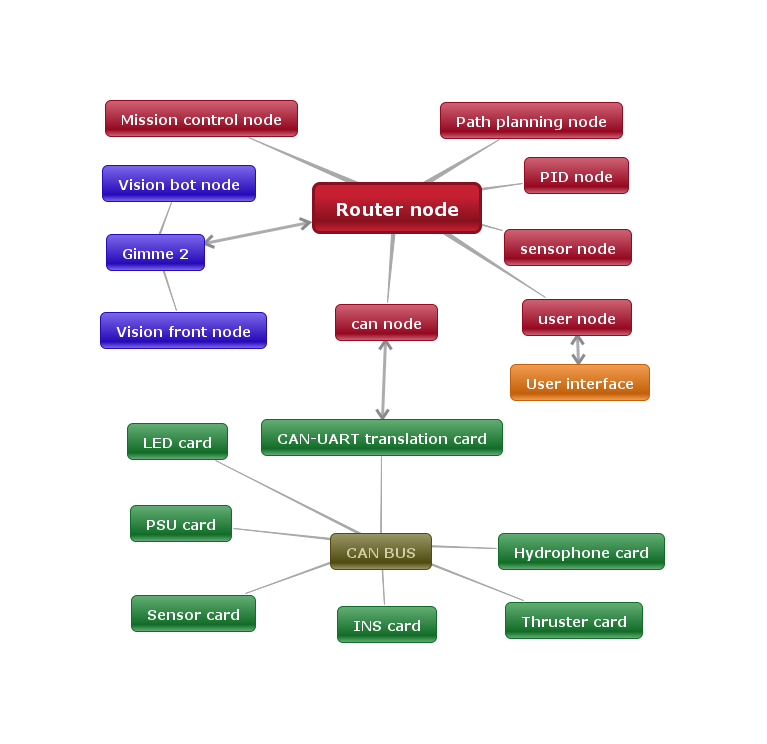
\includegraphics[width=80mm]{./Images/Software/flowchart.png}
		\caption{Complete flowchart of software}
		\label{YourLabel}
	\end{center}
\end{figure}
